\section{Entwurf}
\label{sec:Entwurf}
In der Entwurfsphase sollen aus den Anforderungen Modelle der zu entwickelten Software entstehen, die die konkreten Hardware- und Softwarebezogenen Anforderungen berücksichtigen. Diese Modelle gelten dann als unmittelbare Vorlage für die sich anschließende Implementationsphase. (vgl. \cite[S. 69]{dumke-2003})

UML-Diagramme sind unter anderem ein effektives Werkzeug, um den Programm- und Datenentwurf zu unterstützen und zu dokumentieren. Letztendlich soll mithilfe geeigneter Modelle ein Entwurf der zu Implementierenden Software erarbeitet werden. Dies umfasst die Festlegung des Softwaredesignes, der Datenstruktur und der grafische Oberfläche.

\subsection{Programmentwurf}
\label{sec:Programmentwurf}
Der Programmentwurf bezieht sich auf die Programmlogik \bzw die Funktionalität. Dabei sollen nötige Funktionen des Programms in Abhängigkeiten zueinander dargestellt werden. Für die einzelnen Funktionen wurden Programmablaufpläne erstellt die für die Implementierung genutzt werden sollen. Eine stark vereinfachte version für den änderungsvorgang von Anwesenheiten siehe Anhang \ref{abb:PAP}. Für den überblick des gesamten Prozesses wurde ein Ablaufdiagramm erstellt was die Prozesschritte mit den benötigten Datenquellen zeigt.

\begin{figure}[htb]
    \centering
    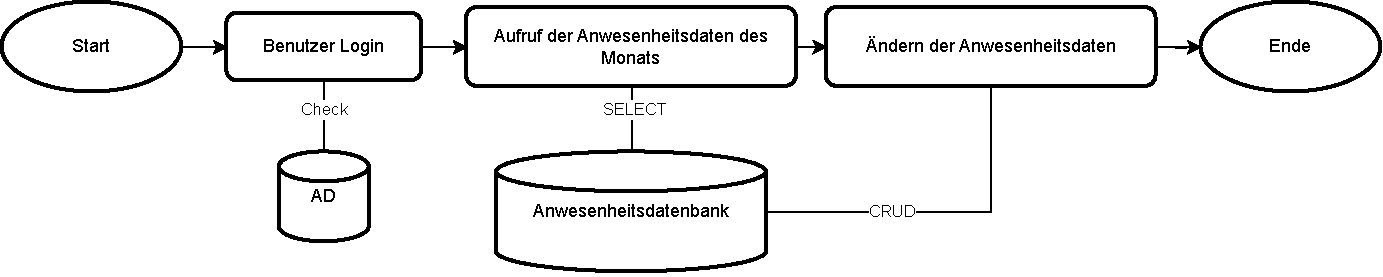
\includegraphics[width=0.9\textwidth,angle=0]{abb/Flow-Diagramm.drawio.pdf}
    \caption[Beschreibung]{Ablaufdiagramm}
    \label{abb:Flow}
\end{figure}

Die Anwendung soll als erstes den Nutzer authentifiezieren um die Berechtigungen feststellen zu können. Wenn der Nutzer berechtigt ist wird seine Referatszugehörigkeit mittels des AD ermittelt. Nach dem Login Prozess werdem dem Nutzer im Frontend die Anweseheitsdaten seiner Kollegen das aktuellen Monats angezeit. Dort kann er seine eigenen Anwesenheiten ändern oder in den Monatsansichten vor und zurück springen. Jede änderung eines eigenen oder im Falle eines Admins, eines Datensatzes im generellen wird direkt an die Datenbank übermittelt und dort gespeichert.


\subsection{Datenentwurf}
\label{sec:Datenentwurf}
Die Einbindung einer Datenbank erfordert ebenfalls einen detaillierten Programmentwurf. UML-Diagramme wie das ERM können verwendet werden, um die Tabellenstruktur, die Beziehungen zwischen den Tabellen und die Attribute zu modellieren. Dies ermöglicht eine klare Darstellung der Datenbankstruktur und hilft dabei, die Datenintegrität und -konsistenz sicherzustellen. Durch diese Art an Dokumentation ist es auch möglich bei der Entwicklung des Programms passende Klassen für die verarbeitung der Daten aus der Datenbank herzuleiten.

Die zuspeicherten Daten ergeben sich aus der in der Analysepahse erhoben Tabelle im Abbildung \ref{abb:Ausgangstabelle}. Um die Daten einfach aus der Datenbank auslesen und zurückschreiben zu können, sollte versucht werden die Datenstruktur so anzulegen das die Daten in einer für die Logik gut verarbeitsbares Schema gespeichert werden. Um die Daten für den Benutzer anzuzeigen müssen die in der Datenbank gespeicherten Daten dann in Objekte zurückgewandelt werden. Um eine möglichst einfache Konvertierung zu ermöglichen wurde auf eine Normalisierung der Tabellenstruktur verzichtet.
%TODO:ERD mit erklärung

